\begin{table}[H]
\centering
\begin{tabular}{@{}lll@{}}
\toprule
\textbf{Aspekt} & \textbf{Axion} & \textbf{Elektron} \\ \midrule
Masse & \(10^{-5}\) eV & 511 keV \\
Wellenlänge & \(0,124\) m & \(2,4\times10^{-12}\) m \\
Verhalten & Welle & Teilchen \\
Wechselwirkung & Sehr schwach & Elektromagnetisch \\
Rolle in ART-12D & Mode des Akasha-Feldes & Neuronaler Empfänger \\ \bottomrule
\end{tabular}
\end{table}

\subsection{Was für Teilchen durchqueren Ihren Körper?}
Die Dunkle Materie hat eine lokale Dichte von etwa 0,3 GeV/cm$^3$ (Read, 2014). Die Anzahldichte hängt jedoch von der Masse ab, $n = \rho/m$, und der Fluss ist $\Phi = n v$. Für eine Mode von $10^{-5}$ eV und $v = 300$ km/s ergibt sich:
\begin{equation}
n = \frac{0,3 \times 10^{15}\ \text{eV/m}^3}{10^{-5}\ \text{eV}} = 3,0\times10^{19}\ \text{m}^{-3},
\qquad
\Phi = n v = 9,0\times10^{24}\ \text{m}^{-2}\text{s}^{-1}.
\end{equation}
Für einen menschlichen Körper mit einer Oberfläche von 0,7 m$^2$:
\begin{equation}
\Phi_{\text{body}} = 9,0\times10^{24} \times 0,7 \approx 6\times10^{24} \text{ particles/s}.
\end{equation}
Etwa $6\times10^{24}$ Teilchen pro Sekunde. (Version 30 behauptete $n = 3000$ m$^{-3}$ und $6\times10^8$ s$^{-1}$; jene Werte entsprechen einem WIMP von etwa 100 GeV, nicht einer Mode von $10^{-5}$ eV.)

\begin{figure}[H]
\centering
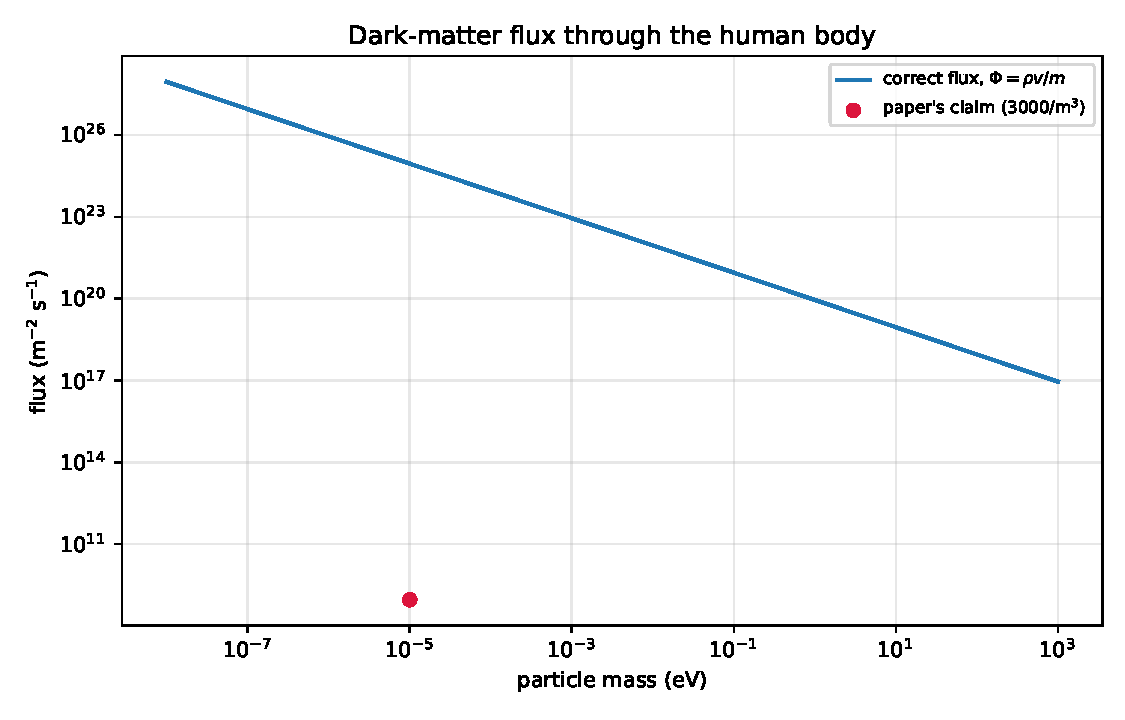
\includegraphics[width=0.82\textwidth]{figures/fig07_flux.pdf}
\caption{Der Fluss der Dunklen Materie durch den menschlichen Körper in Abhängigkeit von der Teilchenmasse. Der rote Punkt markiert die Aussage der Version 30; die Kurve ist der korrekte Wert für $\rho = 0,3$ GeV/cm$^3$ und $v = 300$ km/s. Bei $10^{-5}$ eV beträgt der Unterschied 16 Größenordnungen.}
\label{fig:flux}
\end{figure}

\subsection{Was geschieht mit diesen Teilchen?}
Die meisten durchdringen Sie, ohne wechselzuwirken. Einige wechselwirken mit Atomkernen: spinunabhängig ($\sim 5$ Kollisionen/Jahr), spinabhängig ($\sim 30$ Kollisionen/Jahr). Die Wirkung auf den Körper: natürliche Strahlung ($\sim 2,4$ mSv/Jahr); Dunkle Materie ($\sim 10^{-15}$ mSv/Jahr).

\subsection{Wie weisen wir diese Teilchen nach?}
Direkte Detektoren: LUX-ZEPLIN (10 Tonnen Xenon) --- Empfindlichkeit: $10^{-48}$ cm$^2$. Indirekte Detektoren: Fermi-LAT (sucht Gammastrahlen aus Annihilation), ADMX (sucht Axionen). Wirkungsquerschnitt: $\sigma \sim 10^{-47}$ cm$^2$. Wechselwirkungswahrscheinlichkeit: $P \sim 10^{-22}$.

\subsection{Dunkle Materie als Welle, nicht als Teilchen}
Wenn die Dunkle Materie ein Skalarfeld ist, dann besteht sie nicht aus einzelnen Teilchen. Sie ist eine Welle, die das Universum erfüllt. Formalisierung: $A(x,t) = \sum_n A_n \cos(\omega_n t + \varphi_n)$.

\subsection{Die Analogie von Baum und Photon}
Stellen Sie sich einen Baum an einem Strand vor. Die Sonne scheint. Photonen verlassen die Sonne mit der Energie $E = h\nu$. Sie erreichen den Baum. Sie werden von jedem Blatt mit derselben Energie $h\nu$ absorbiert. Wie kann ein einzelnes Photon alle Blätter mit derselben Energie erreichen? Wäre es ein Teilchen, würde es bei jeder Kollision Energie verlieren. Das tut es aber nicht. Die Antwort ist einfach: Weil das Photon eine Welle ist, kein Teilchen. Eine Welle wird nicht „verbraucht``, wenn sie Materie durchläuft. Sie breitet sich über den gesamten Raum aus. Jedes Blatt „sieht`` die ganze Welle. Der Zustand des Photons: $|\psi_{\text{photon}}\rangle = \int d^3k \, c(k) |k\rangle$.

\subsection{Welle-Teilchen-Dualität als Durchquerungsmechanismus}
Wenn Materie nicht zwischen Universen wechseln kann (weil das unendliche Energie erfordern würde) und die Universen über die Dunkle Materie verbunden sind, wie kommunizieren sie dann? Die ART-12D-Antwort: über die Welle-Teilchen-Dualität. Schritt 1: Die Materie wird zur Welle. $|\text{particle}\rangle_A \to |\text{wave}\rangle_A$. Schritt 2: Die Welle geht hinüber. $|\text{wave}\rangle_A \to |\text{wave}\rangle_B$. Schritt 3: Die Welle wird zum Teilchen. $|\text{wave}\rangle_B \to |\text{particle}\rangle_B$. Schritt 4: Die Information wird umgesetzt. $I_A \to I_B$.

\subsection{Das menschliche Gefühlsspektrum}
Menschliche Gefühle fallen in zwei große Kategorien: positive und negative. Jedes Gefühl hat eine charakteristische Frequenz und eine spezifische Wirkung auf das Bewusstsein. Formalisierung: $S_{\text{total}} = \sum_{i=1}^{48} S_i^{\text{positive}} + \sum_{j=1}^{46} S_j^{\text{negative}}$. Hier ein Auszug aus der erweiterten Tabelle (die vollständige Fassung findet sich in Anhang B):
\begin{table}[H]
\centering
\begin{tabular}{@{}lll@{}}
\toprule
\textbf{Gefühl} & \textbf{Dominante Frequenz (Hz)} & \textbf{Wirkung} \\ \midrule
Freude & 400-600 & Ausdehnung, Dynamik \\
Frieden & 200-350 & Reflektierte Ruhe \\
Liebe & 200-400 & Tiefe Emotion \\
Dankbarkeit & 300-500 & Zufriedenheit \\
Angst & 500-800 & Aktiviert die Amygdala \\
Wut & 600-800 & Zorn \\
Trauer & 400-600 & Melancholie \\
Neid & 600-800 & Eifersucht \\ \bottomrule
\end{tabular}
\end{table}
Die therapeutischen Musikfrequenzen (432 Hz, 528 Hz, 639 Hz, 741 Hz, 852 Hz, 963 Hz) wurden mit den Frequenzen des Akasha-Feldes in Beziehung gesetzt. Die sieben menschlichen Sinne umfassen fünf physische (Sehen, Hören, Riechen, Schmecken, Tasten) und zwei geistige (Vorstellungskraft, Empathie).

\subsection{Das Herz als Modulator des Empfangs}
Das Herz besitzt ein eigenes elektrisches System (den Sinusknoten), das Impulse unabhängig vom Gehirn erzeugt. Es wirkt als Modulator des Empfangs, nicht als unabhängiger Empfänger. Das Gehirn ist der Hauptempfänger, das Herz justiert die Kohärenz. Formalisierung: $C_{\text{coherent}} = C_0 \times (1 + \beta \times HRV)$. Die genauen wissenschaftlichen Zahlen: Das Gehirn verbraucht etwa $20$ W Stoffwechselleistung, das Herz erbringt etwa $1-1,3$ W mechanische Leistung, erzeugt aber elektrische und magnetische Felder deutlich größerer Amplitude.

\subsection{Das Wort, das jede Medizin ersetzen kann}
Die Hypothese: $L_{\text{word-matter}} = g_{CM} A_{\text{meaning}} \psi \psi$. Was das Wort bewirken kann: $Effect_{\text{total}} = Effect_{\text{medicine}} + Effect_{\text{word}} + \text{Interaction}$. Was das Wort nicht bewirken kann: Es kann keine Antibiotika bei bakteriellen Infektionen ersetzen, kein Insulin bei Typ-1-Diabetes, keine Operation bei Blinddarmentzündung, keine Chemotherapie bei Krebs. Vorhersage 67: die Wirkung des Wortes.

\newpage
